\documentclass[twocolumn,twoside,10pt,a4paper]{article}

\usepackage[english]{babel}  % portuguese
\usepackage{graphicx}           % images: .png or .pdf w/ pdflatex; .eps w/ latex

%% For iso-8859-1 (latin1), comment next line and uncomment the second line
\usepackage[utf8]{inputenc}

\usepackage{times}              % PS fonts
\usepackage[T1]{fontenc}        % T1 fonts
%\usepackage{lastpage}           % to have lastpage in headers
\usepackage{url}                % urls

% geometry package
\usepackage[outer=20mm,inner=30mm,vmargin=20mm,includehead,includefoot,headheight=15pt]{geometry}

%% space between columns
\columnsep 10mm

% avoid widows and orphans
\clubpenalty=300
\widowpenalty=300

\usepackage[pdftex]{hyperref}
\hypersetup{%
    a4paper = true,              % use A4 paper
    bookmarks = true,            % make bookmarks
    colorlinks = true,           % false: boxed links; true: colored links
    pdffitwindow = false,        % page fit to window when opened
    pdfpagemode = UseNone,       % do not show bookmarks
    pdfpagelayout = SinglePage,  % displays a single page
    pdfpagetransition = Replace, % page transition
    linkcolor=blue,              % hyperlink colors
    urlcolor=blue,
    citecolor=blue,
    anchorcolor=green
}

\usepackage{indentfirst}       % indent also 1st paragraph

\pagestyle{myheadings}         % Option to put page headers
\markboth{{\small\it Scalable Vector Graphics}}
{{\small\it Group 08, \today}}

%\hyphenation{}                  % explicit hyphenation

% entities
\newcommand{\class}[1]{{\normalfont\slshape #1\/}}
\newcommand{\svg}{\class{SVG}}
\newcommand{\scada}{\class{SCADA}}
\newcommand{\scadadms}{\class{SCADA/DMS}}

\title{Scalable Vector Graphics}

\author{João Gradim\\
\small Faculdade de Engenharia da Universidade do Porto,\\[-0.8ex]
\small R.\ Dr.\ Roberto Frias, 4200-465 Porto\\[-0.8ex]
\small \texttt{ei05030@fe.up.pt}\\
\and
Nuno Polónia\\
\small Faculdade de Engenharia da Universidade do Porto,\\[-0.8ex]
\small R.\ Dr.\ Roberto Frias, 4200-465 Porto\\[-0.8ex]
\small \texttt{ei05037@fe.up.pt}
}

\date{\today}

\begin{document}

\maketitle
\thispagestyle{plain}

\begin{abstract}
The purpose of this article is to give a short description of SVG, covering its history, purpose and syntax. Chapter 1 gives a small introduction to SVG and compares vector to raster images. Chapter 2 presents two other vector image markup languages from which SVG derived. Chapter 3 describes the main XML concepts behind the SVG implementation and Chapter 4 describes the validation methods for both SVG 1.1 and SVG 1.2. Finally, chapter 5 presents final remarks regarding the contents of this article\\
\end{abstract}

%http://www.dmoz.org/Computers/Data_Formats/Graphics/Vector/SVG/
\section{Introduction}\label{sec:intro}
Scalable Vector Graphics (SVG) is an XML markup language specification for describing two-dimensional vector graphics.\\
W3C started developing it in 1999 after Adobe and Microsoft submitted two different and competing standards, the Precision Graphic Markup Language (PGML) and the Vector Markup Language (VML) respectively, both in 1998.\\

\subsection{Vector and Raster Graphics}
Vector graphics rely on the use of mathematical equations to describe geometrical primitives from which the images are made of. This allows them to be scaled to a larger or smaller size without any quality loss (see Figure \ref{fig:vector_vs_raster}). Edition is also easier because every new point can be recalculated. Raster images, or bitmaps, are made up of a data structure composed of pixels which have color and position information. These kind of images have no semantic meaning, and a pixel is an entity by itself: it has no ``self-awareness''  and what kind of object or objects it is part of. On the contrary, SVG and most vector image formats are defined in a way that allows their composing elements to be freely and independently manipulated without interfering with other parts of the image.

\begin{figure}[h]
\centering
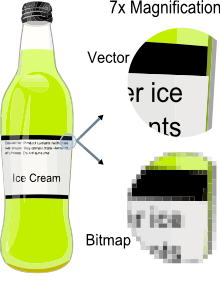
\includegraphics[width=40mm]{images/vector_bitmap.png}
\caption{Vector Image vs Raster Image}
\label{fig:vector_vs_raster}
\end{figure}

\section{XML Vector image formats}

%http://en.wikipedia.org/wiki/List_of_vector_graphics_markup_languages
\subsection{Precision Graphics Markup Language (PGML)}

PGML first appeared in 1998, as an initial draft proposed to W3C, despite of not being adopted as a recommendation\cite{w3c:pgml}. PGML is a 2D XML-based vector drawing language and uses the imaging model of the PostScript language and PDF as its basis in order to provide simple-to-use graphical objects and precise visual fidelity.

\subsection{Vector Markup Language (VML)}

As with PGML, VML was submitted as a proposed standard to the W3C in 1998 by Autodesk, Hewlett-Packard, Macromedia, Microsoft, and Visio.\\

VML was designed to support the markup of vector graphic information in the same way that HTML supports the markup of textual information. Within VML the content is composed of paths described using connected lines and curves. The markup provides both semantic and presentation information about these paths.\\

VML is mainly used by Microsoft and its related products, such as Microsoft Word and Internet Explorer.

\section{SVG}

SVG is a royalty-free, vendor-neutral open standard developed under the W3C (World Wide Web Consortium) Process, with a strong development support by Adobe and other major companies.\\
The SVG specification is an open standard that has been under development by the World Wide Web Consortium (W3C) since 1999. There are three different SVG specifications: 1.0, 1.1, 1.2 Tiny. The current, and most widely adopted is 1.1, as 1.2 is still a working draft.\cite{w3c_svg}

\subsection{Model Description}

Being an XML language, SVG benefits from techniques and technologies applicable to other XML documents, such as XSLT transformations, embedding an SVG document in another XML documents using namespaces and even styling through CSS stylesheets.\\

SVG is composed of three types of graphical objects: Vector images, Raster images and Text.\\

Graphical objects can be grouped, styled, transformed, and composited into previously rendered objects. Text can be in any appropriate XML namespace, which enhances searchability and accessibility of the SVG graphics. The feature set includes nested transformations, clipping paths, alpha masks, filter effects, template objects and extensibility.\cite{eisenberg}

\subsection{Elements}

SVG uses both self-closing and content elements. For example, a \verb!<rect>! element is defined solely based on its attributes, such as \verb!width! and \verb!height!, and does not need any content to describe it. However, a series of \verb!<rect>! elements may be part of a \verb!<g>! (group) element. This is because a group element only makes sense when it groups a series of elements as its content.\\

A full reference of all the SVG 1.1 elements may be found at \url{http://www.w3schools.com/svg/svg_reference.asp}

%http://www.w3schools.com/svg/svg_reference.asp
%http://www.w3.org/TR/SVGTiny12/types.html
%http://www.w3.org/TR/SVGTiny12/struct.html

\subsection{Attributes}

Attributes are a big part of the SVG specification. As SVG is a language that describes a drawing (composed by a series of graphical elements, such as rectangles, ellipses, and others) as an XML document, most of its elements are described by their attributes and their respective values. This is because, as in most XML languages, content describes \textbf{data} associated with that element and attributes describe the \textbf{metadata} for that element. One notable exception are SVG paths, which describe their contents not as nested elements, but as a series of space-delimited numbers in a single attribute.\cite{ibm_xml}

\section{Schema}

The current SVG specification, SVG 1.1, has a DTD available for validation. As such, a stand-alone SVG document using this specification should have the correct DOCTYPE definition (see Annex 1) specified to be considered a valid SVG document.\\

As SVG 1.2 does not have a DTD\cite{svg_no_dtd}, it is not necessary to specify a DOCTYPE. There is, however, a schema available for validation based on the RelaxNG schema\footnote{RelaxNG is a namespace-aware schema language that uses the datatypes from XML Schema Part 2. This allows namespaces and modularity to be much more naturally expressed than using traditional DTD syntax.}

\section{SVG Applications}

A lot of popular vector imaging edition programs like Adobe Illustrator or Inkscape use the SVG format as its basis.\\

With Web 2.0, as the websites became more and more complex, SVG became a versatile way of showing or working with complex shapes so nowadays every major web browser (except for Internet Explorer 8.0 and below) has its own SVG rendering implementation.\\


\section{Final Remarks}

After reading this study, one should not despise raster imaging as it has its advantages too. Raster images Vectorial and raster graphics should be looked at as complementary and not competing types.\\

As for SVG, it is a heavily documented, greatly supported markup language for representing vectorial images. It is extremely versatile, being able to be used for both on-screen and print with losing any quality.\\

%% auto bibliographic list 
\renewcommand{\bibname}{References}
\bibliographystyle{unsrt-pt}
\bibliography{lapd1}

\newpage
\ \\
\newpage
\section*{Annex 1: SVG 1.1 DOCTYPE}\label{sec:svg11doctype}
\tiny{
\begin{verbatim}
<!DOCTYPE svg PUBLIC "-//W3C//DTD SVG 1.1//EN"
	"http://www.w3.org/Graphics/SVG/1.1/DTD/svg11.dtd">
\end{verbatim}
}

\end{document}


